\documentclass[a4paper, 10pt]{article}
\usepackage[margin = 1in]{geometry}
\usepackage{amsmath}
\usepackage{tabularx}
\usepackage{framed}
\setlength{\parindent}{0em}
\newcolumntype{L}{>{\arraybackslash}m{10cm}}
\newcolumntype{T}{>{\arraybackslash}m{6cm}}
\usepackage{graphicx}
\usepackage{pdfpages}

\begin{document}

\section*{Topic 15 - DC Circuits}

\section{Series and parallel arrangement}
\subsection{Equivalent resistance}
\begin{framed}
   It is possible to replace a \textbf{combination of resistors} in any given circuit with a single resistor without altering the p.d. and the current across the terminals of the combination. The resistance of the single resistor is called the \textbf{equivalent resistance} of the combination
\end{framed}	

\subsection{Resistor in series}
The current $I$ through each resistor is the same
\begin{center}
   \begin{framed}
      \[
      R = R_1 + R_2 + R_3 + ... R_n
      \]
      
   \end{framed}	
\end{center}	

\subsection{Resistor in parallel}
The pd.d $V$ through each resistor is the same
\begin{center}
   \begin{framed}
      \[
      \frac{1}{R} = \frac{1}{R_1} + \frac{1}{R_2}+ \frac{1}{R_3 }+ ... \frac{1}{R_n}
      \]
   \end{framed}	
\end{center}	

\subsection{Combination of E.M.F. cells in series}
\[
   E_{tota} = E_1 + E_2
\]

\subsection{Combiantion of E.M.F. cells in parallel}
For two cells with emf $E_1$ 
\[
   E_{total} = E_1
\]


\section{Potential divider}
For a circuit with emf $V_s$ and 2 external loads $R_1$  and $R_2$ and current $I$  \\
The current is given by
\[
I = \frac{V_s}{R_1 + R_2}
\]
The potential difference across $R_1$ is thus
\[
   V_{\circ} = IR_1 = \left( \frac{R_1}{R_1 + R_2} \right)  V_s
\]

\section{Potentiometer}
\subsection{Working principles of a potentiometer}
For the circuit below, $I = 0$ when $E_1 = E_2$
\begin{center}
   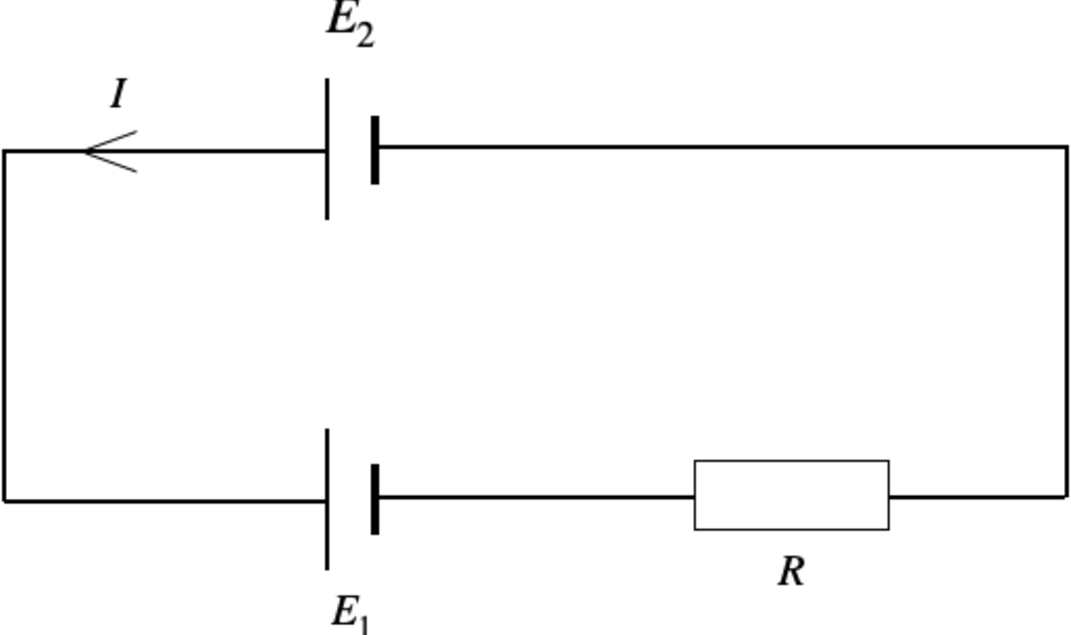
\includegraphics[trim = 50 50 50 50, width=3cm]{figures/1.pdf} 
\end{center}	

Replacing $E_2$ with a potential divider circuit,  \\
\begin{center}
   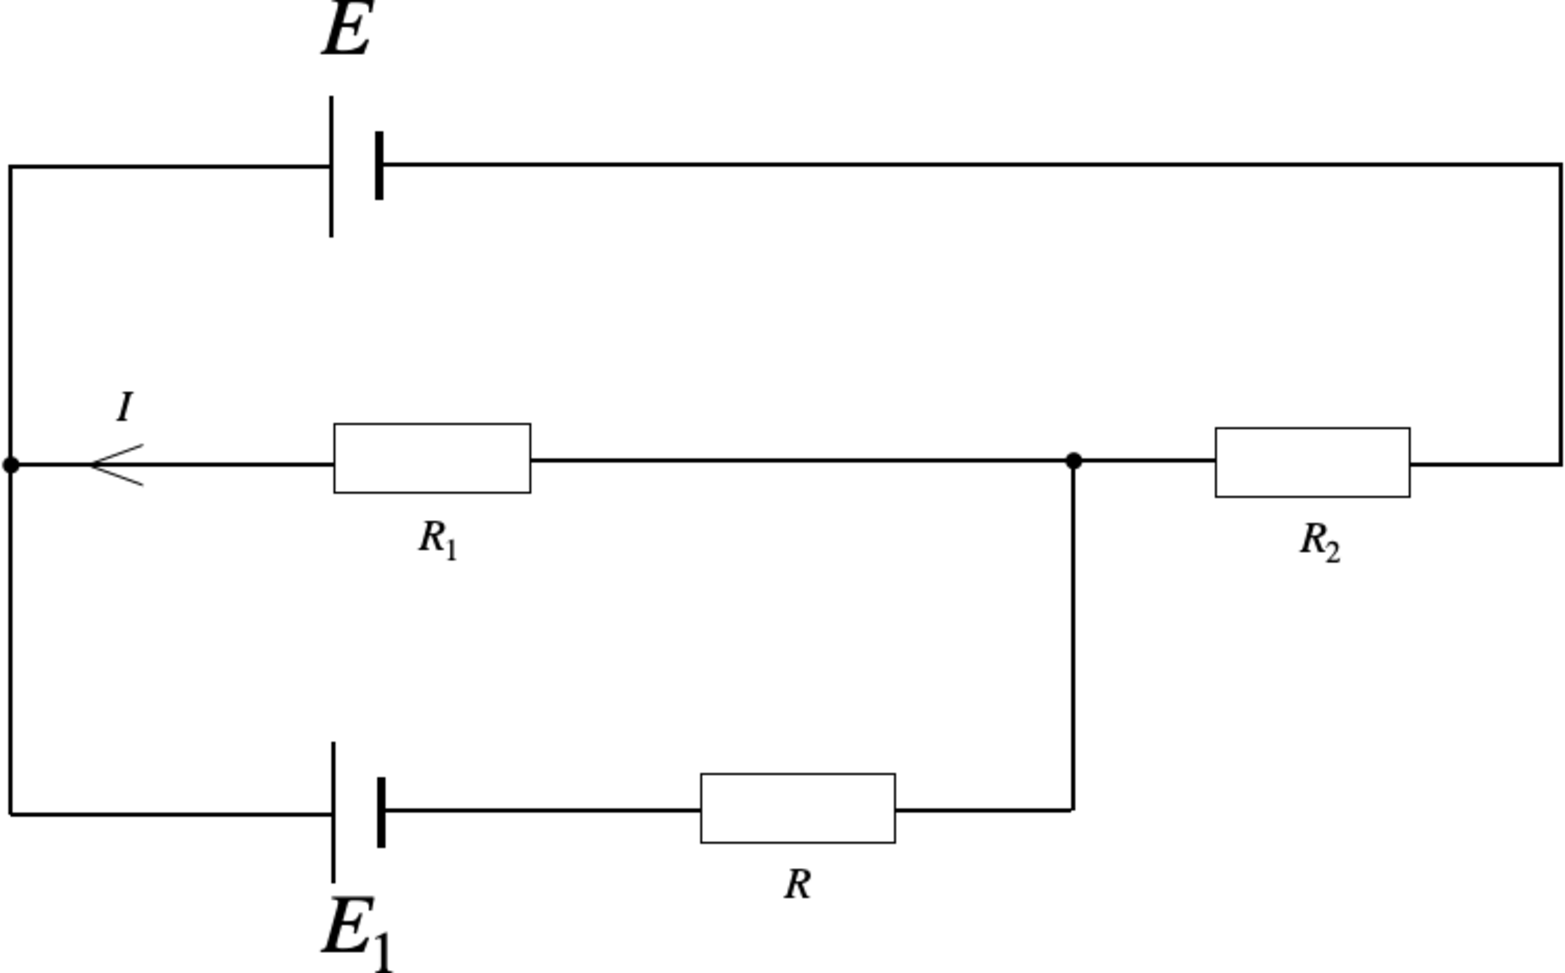
\includegraphics[width=3in]{figures/2.pdf}  
\end{center}	

By varying $R_1$ and $R_2$, no current flows through $E_1$ when the $p.d.$ across $R_1$ is equal to $E_1$ 


\subsection{Null point, balance point and balance length}
By replacing $R_1$ and $R_2$ with a resistance wire $AB$ and a sliding contact at point $C$, the galvanometer shows no reflection at \textbf{null point} or \textbf{balance point}. $AC$ is the \textbf{balance length}. \\

\begin{center}
  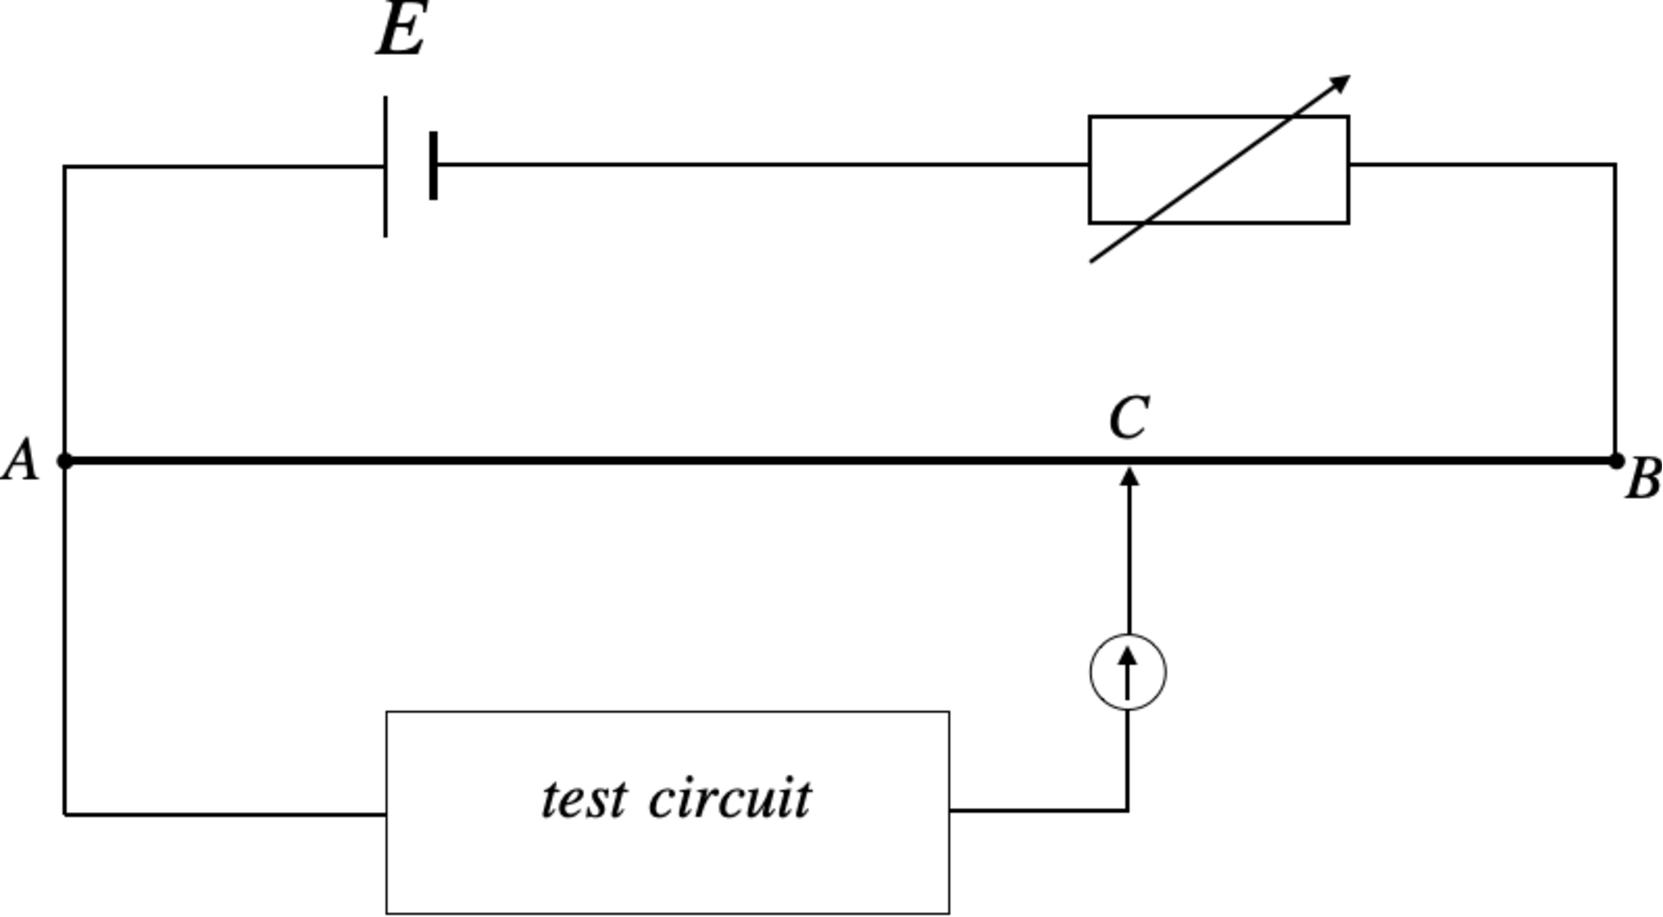
\includegraphics[width=3in]{figures/3.pdf} 
\end{center}	

Assuming 
\begin{itemize}
   \item Wire $AB$ has uniform cross sectional area
   \item Potential difference across wire remains constant with time
\end{itemize}	

For a \textbf{uniform wire} of length $L$,
\[
   R = \frac{\rho L}{A}
\]
\[
R \propto L
\]

The potential difference aross $AC$ is
\[
   V_{AC} = \frac{R_{AC}}{R_{AB}} \times V_{AB}
\]
\[
   V_{AC} = \frac{L_{AC}}{L_{AB}} \times V_{AB}
\]

\subsection{Voltmeter vs potentiometer}
\begin{itemize}
   \item for potentiometer, no errors are introduced by internal resistance of the cells (since no current flows through the cells at balance length
   \item real voltmeter has \textbf{finite resistance}, and hence draws a current from the cell, and lowers the terminal p.d. of the cell when connected
   \item for potentiometer, since \textbf{no current flows at balance point}, the potentiometer can be considered to be a voltmeter with \textbf{infinite resistance} 
\end{itemize}

\subsection{Application 1 - Comparison of e.m.fs}
\begin{center}
   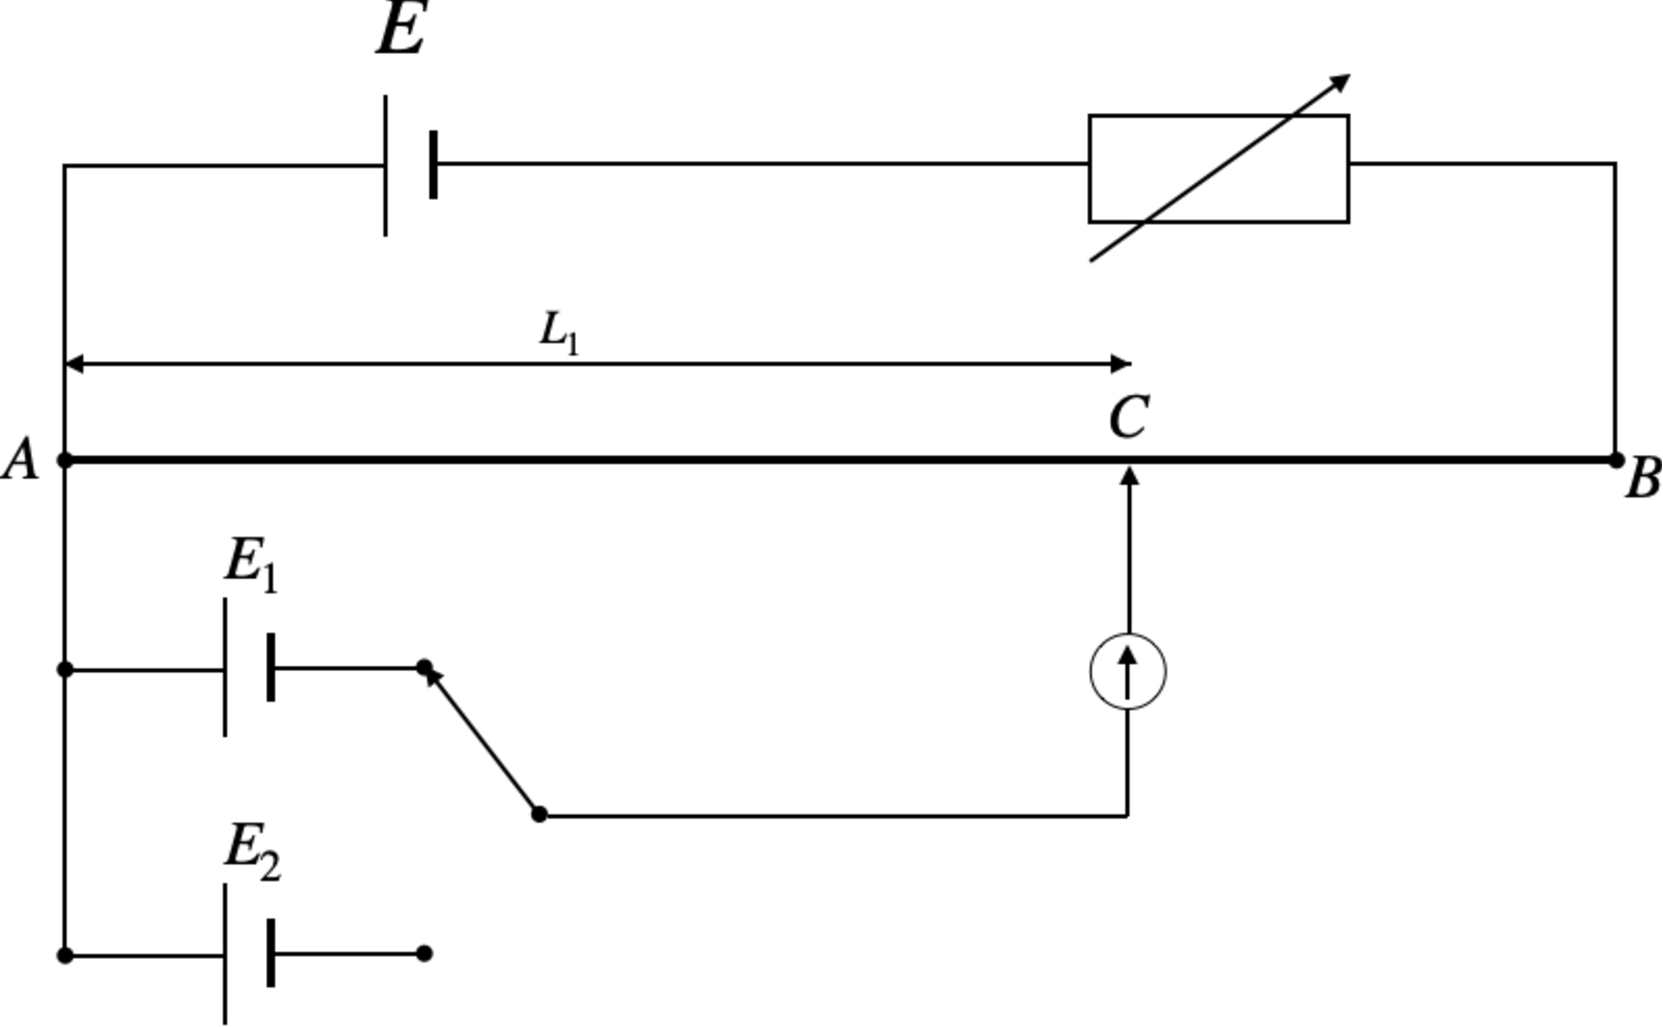
\includegraphics[width=3in]{figures/4.pdf} 
\end{center}	

Since at balance length, 
\[
   E_i = \frac{R_{AC}}{R_{AB}} \times V_{AB}
\]
Since $V_{AB}$ and $R_{AB}$ constant, 
\[
E_i =  k L_i
\]
hence 
\[
\frac{E_1}{E_2} = \frac{kL_1}{kL_2} = \frac{L_1}{L_2}
\]

\subsection*{NOTE - shorting key as a protection for galvanometer}

To ensure precision of potentiometer, the galvanometer used is very sensitive. The galvanometer should be protected from \textbf{high currents} that flows through in \textbf{off-balance} situations, by using a large resistance in series. 

\begin{center}
   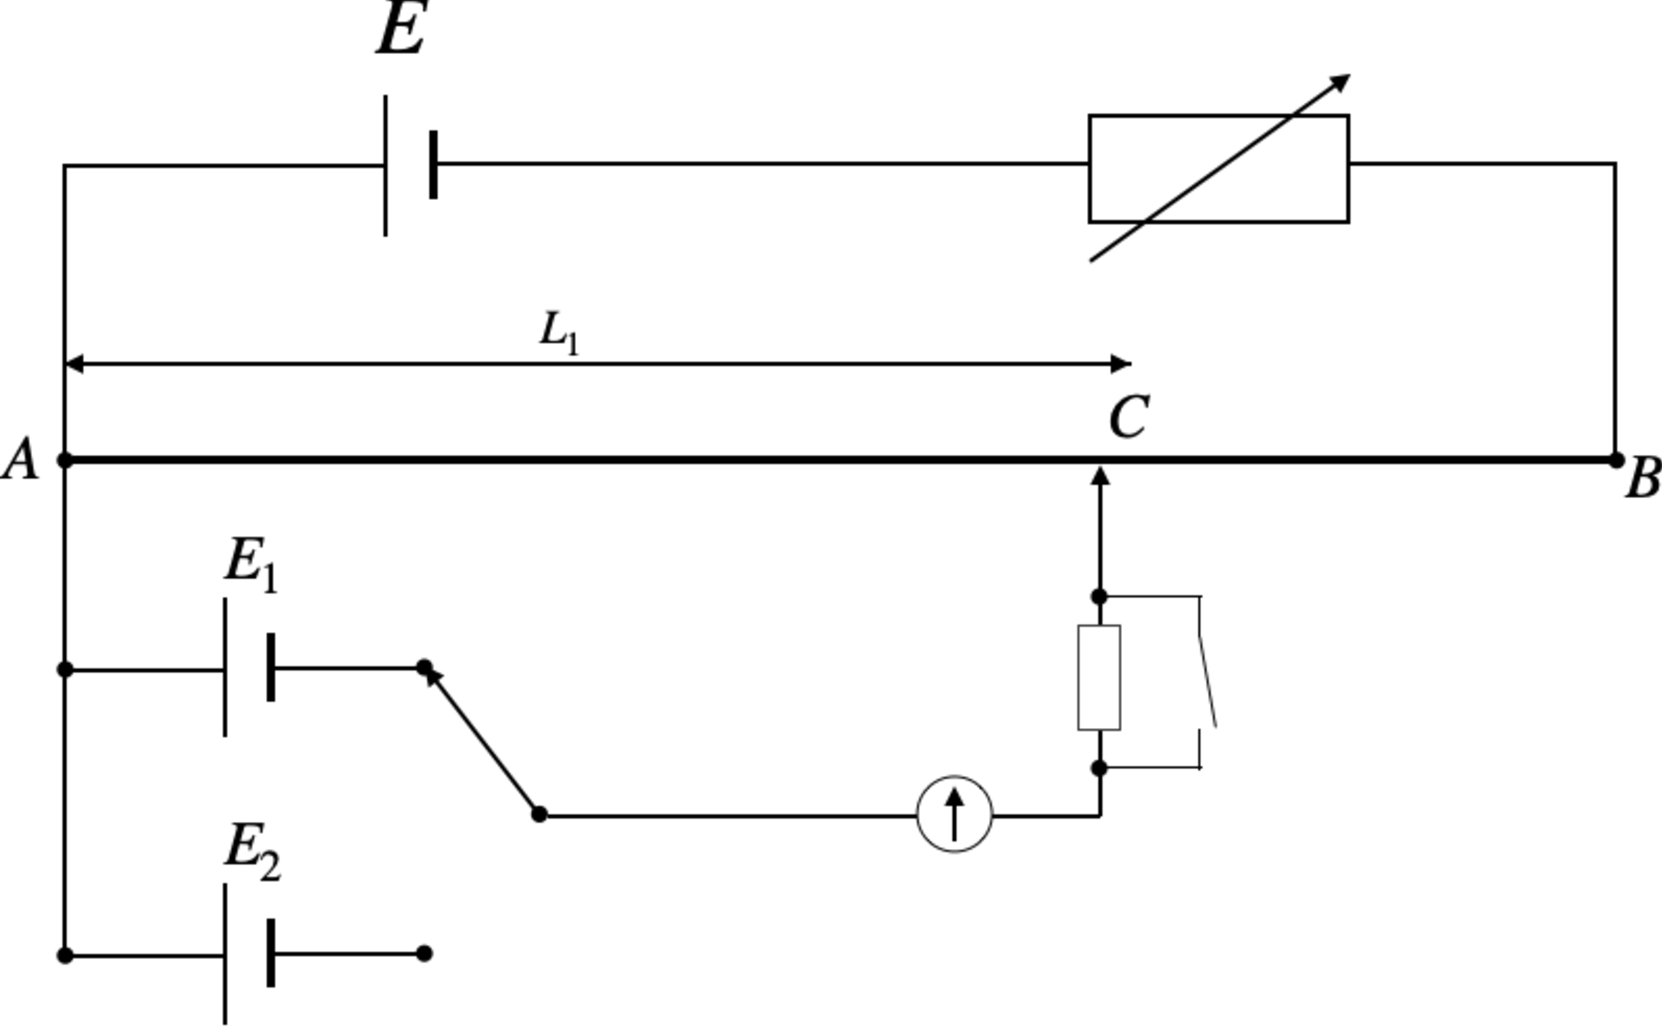
\includegraphics[width=3in]{figures/5.pdf} 
\end{center}	

\begin{itemize}
   \item Before approximate null point is reached, the shorting key is \textbf{left open}, to protect the galvanometer from large currents
   \item nearing the null point, the key is \textbf{closed}, to allow for full current to flow through, so that an accurate balance point can be found
\end{itemize}	

\subsection{Application 2 - Measuring e.m.f. and internal resistance of a cell}
\begin{minipage}{0.5\textwidth}
   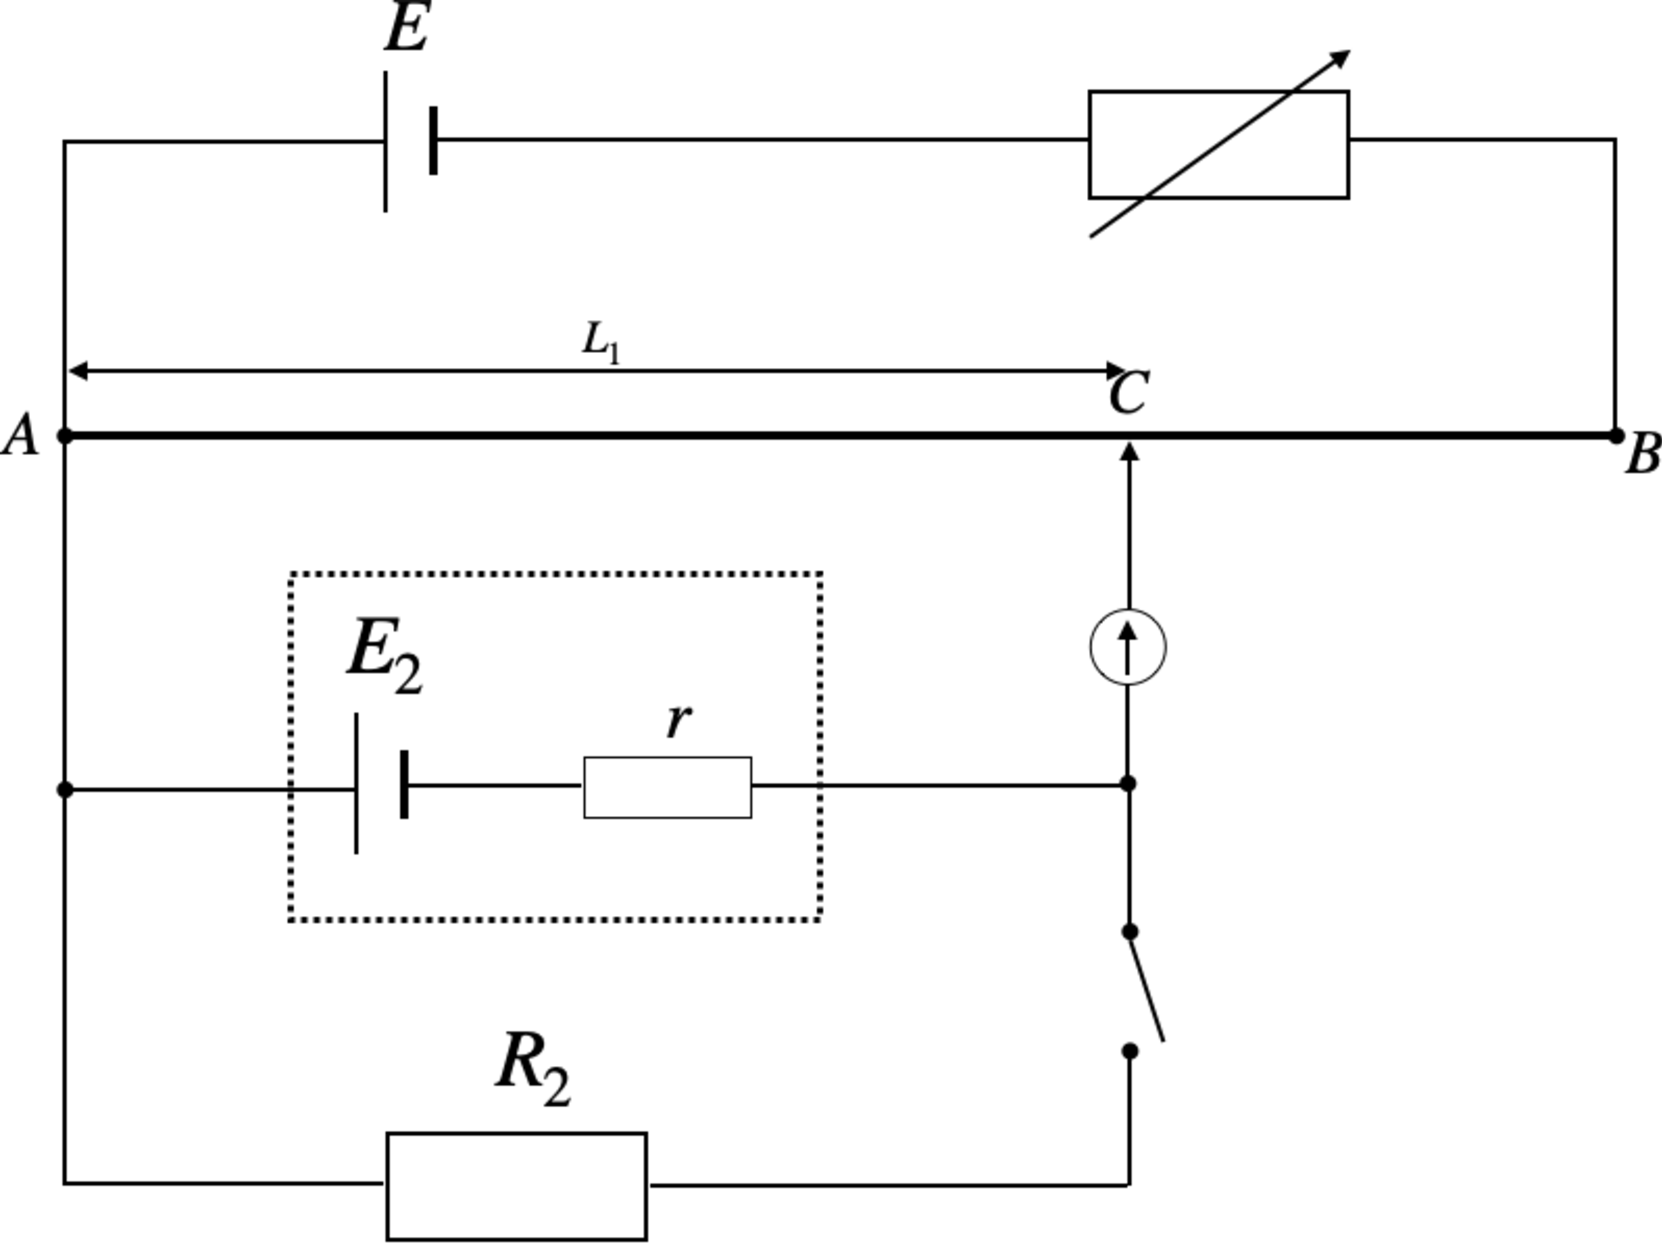
\includegraphics[width=3in]{figures/6.pdf} 
\end{minipage}	
\begin{minipage}{0.5\textwidth}
   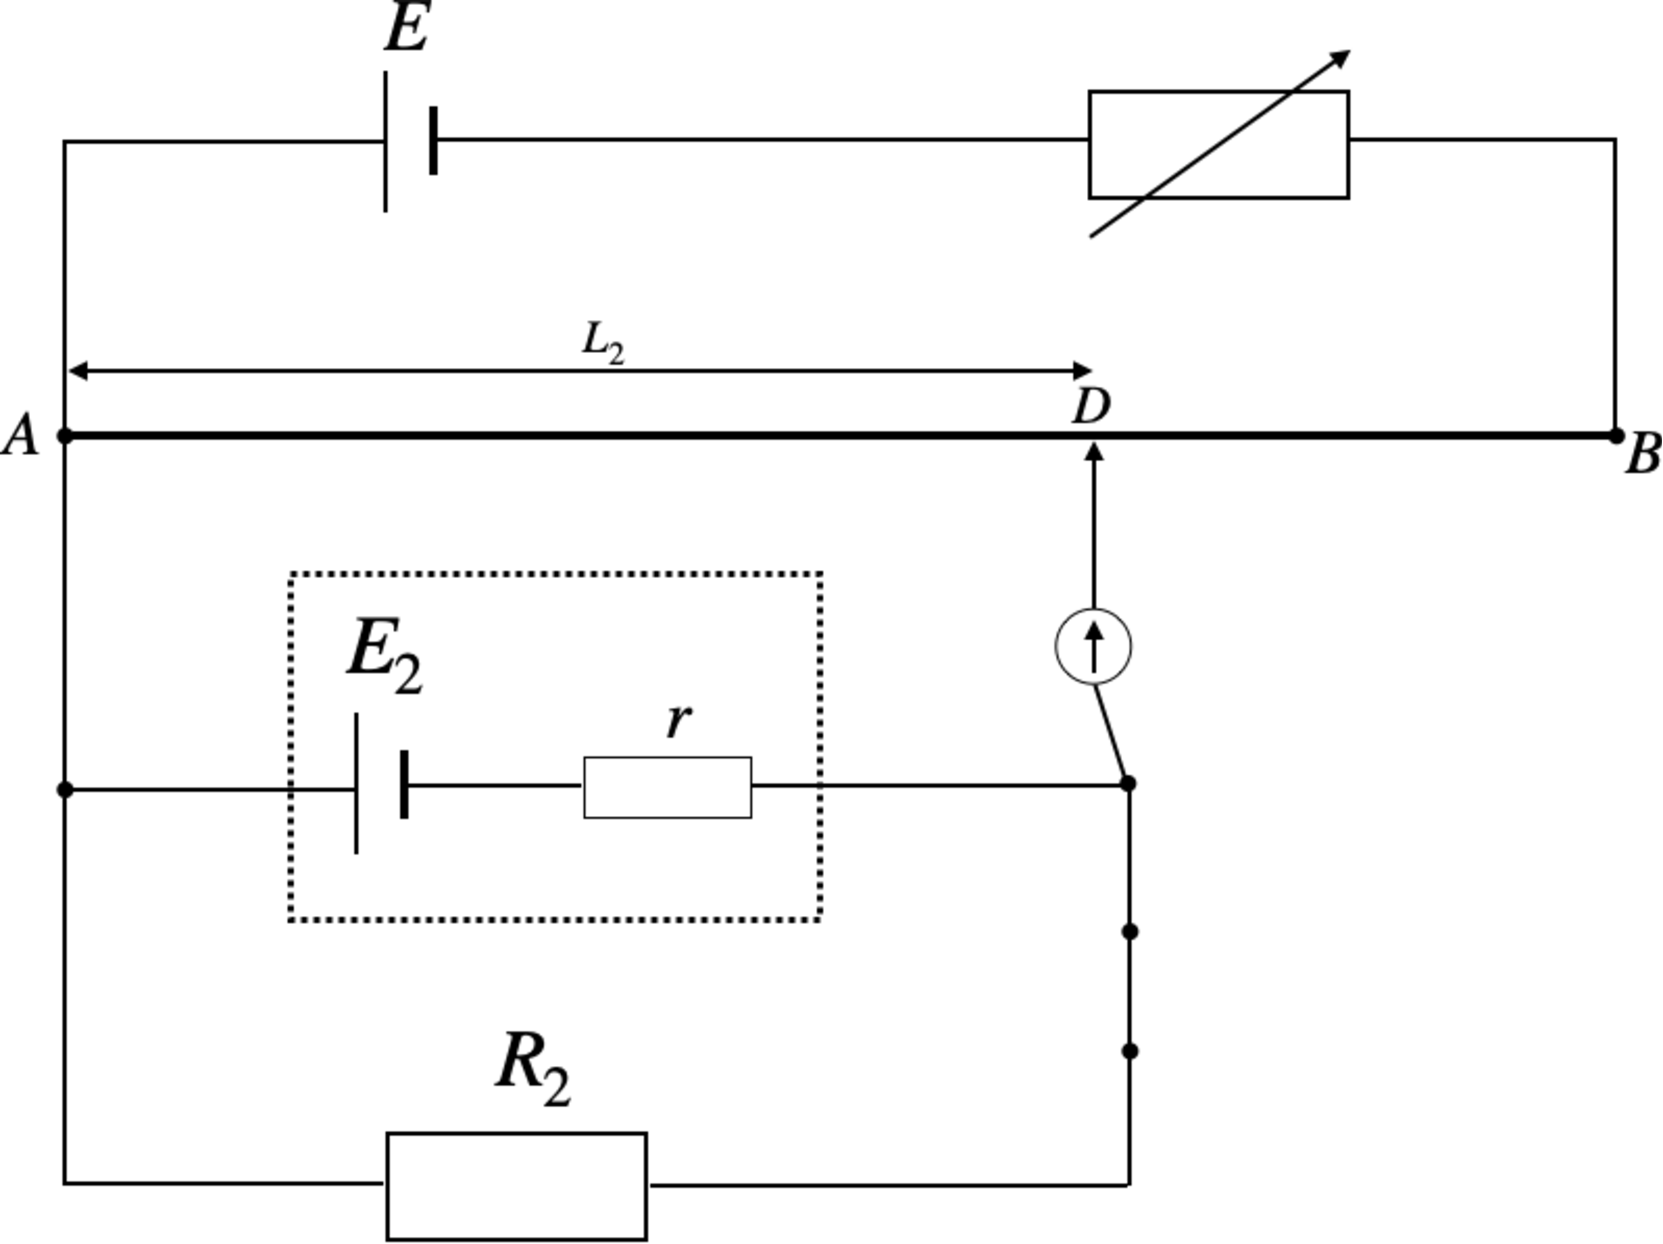
\includegraphics[width=3in]{figures/7.pdf} 
\end{minipage}	

\begin{itemize}
   \item when \textbf{switch is open}, $E_2$ can be found with $L_1$ 
      \[
         E_2 = \frac{L_{1}}{L_{AB}} \times V_{AB}
      \]
   \item when switch is closed, there is a current flowing through $E_2$
      \[
         \text{terminal p.d. across $E_2$} = \text{terminal p.d. across $R_2$} = \frac{L_2}{L_{AB}} \times V_{AB}
      \]
   \item the current flowing through $R_2$ is 
      \[
         I = \frac{V}{R_2} = \frac{L_2}{L_{AB}} \times V_{AB} \times \frac{1}{R_2}
      \]
   \item the internal resistance can be found by 
      \[
      V = E_2 - Ir
      \]
\end{itemize}	

\subsection{Application 3 - Comparison of resistance of two resistors}
\begin{minipage}{0.5\textwidth}
   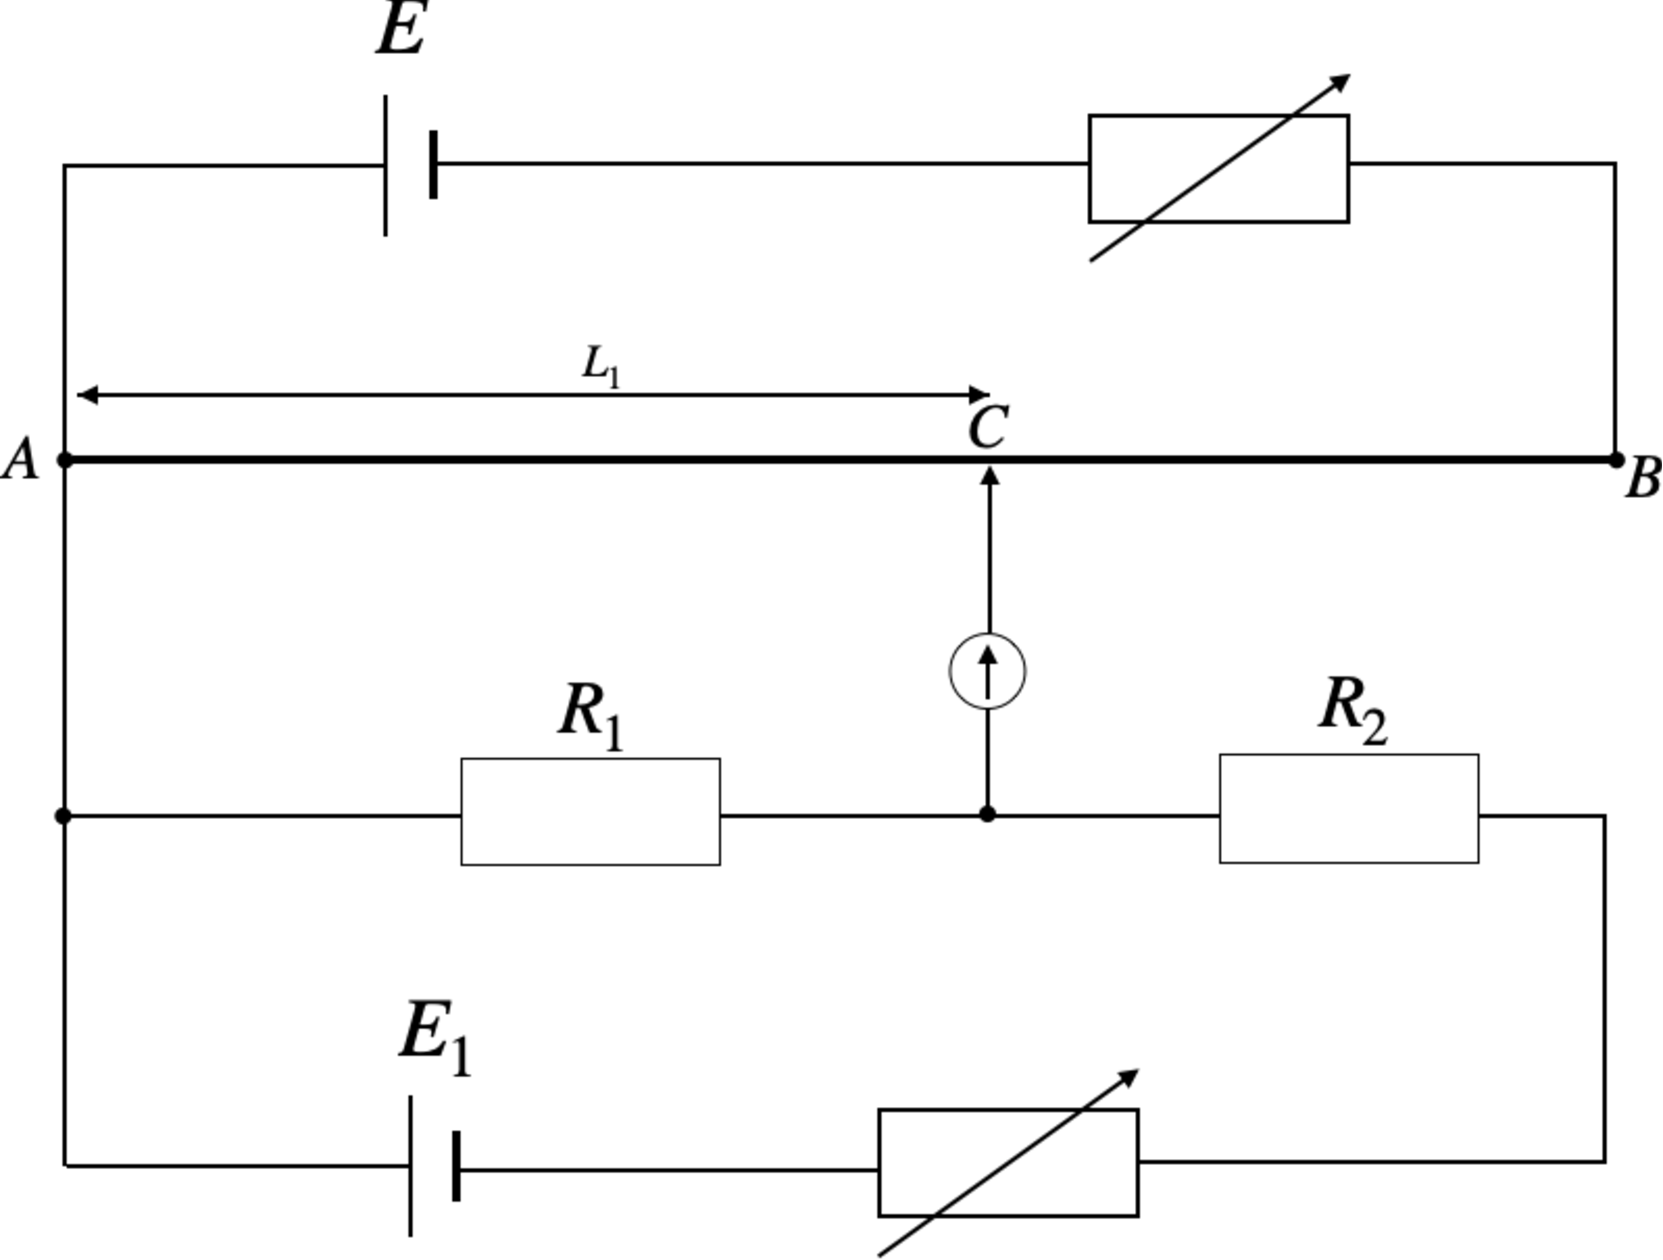
\includegraphics[width=3in]{figures/8.pdf} 
\end{minipage}	
\begin{minipage}{0.5\textwidth}
   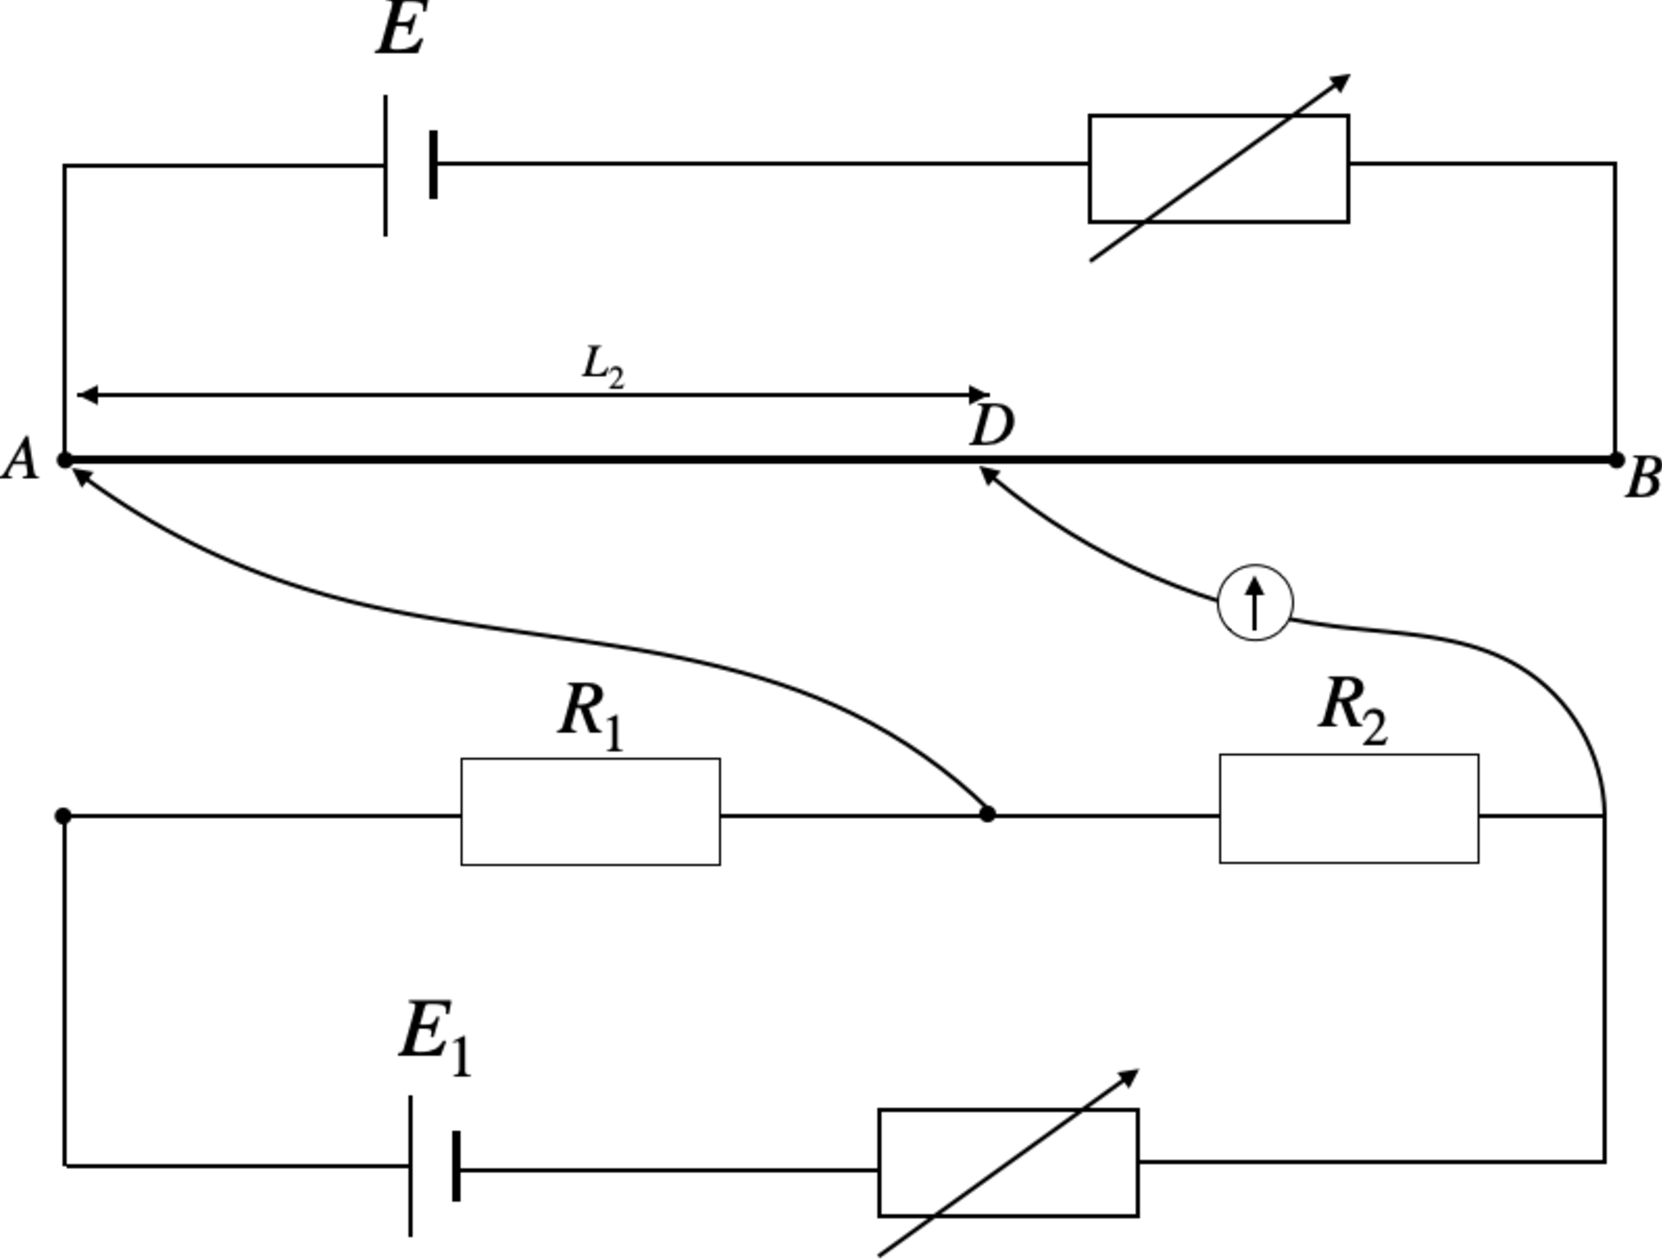
\includegraphics[width=3in]{figures/9.pdf} 
\end{minipage}	

p.d. across $R_1$ is,
\[
   V_1 = \frac{L_1}{L_{AB}} \times V_{AB}
\]
p.d. across $R_2$ is
\[
   V_2 = \frac{L_2}{L_{AB}} \times V_{AB}
\]

hence in the test circuit
\[
   IR_1 = \frac{L_1}{L_{AB}} \times V_{AB}
\]
\[
   IR_R = \frac{L_R}{L_{AB}} \times V_{AB}
\]

since current $I$ is the same
\[
\frac{R_1}{R_2} = \frac{L_1}{L_2} 
\]


















\end{document}	
